%%%%%%%%%%%%%%%%%%%%%%%%%%%%%%%%%%%%%%%%%%%%%%%%%%%%%%%%%%%%%%%%%%%%%%%%%%%%
% AGUtmpl.tex: this template file is for articles formatted with LaTeX2e,
% Modified December 2018
%
% This template includes commands and instructions
% given in the order necessary to produce a final output that will
% satisfy AGU requirements.
%
% FOR FIGURES, DO NOT USE \psfrag
%
%%%%%%%%%%%%%%%%%%%%%%%%%%%%%%%%%%%%%%%%%%%%%%%%%%%%%%%%%%%%%%%%%%%%%%%%%%%%
%
% IMPORTANT NOTE:
%
% SUPPORTING INFORMATION DOCUMENTATION IS NOT COPYEDITED BEFORE PUBLICATION.
%
%
%
%%%%%%%%%%%%%%%%%%%%%%%%%%%%%%%%%%%%%%%%%%%%%%%%%%%%%%%%%%%%%%%%%%%%%%%%%%%%
%
% Step 1: Set the \documentclass
%
%
% PLEASE USE THE DRAFT OPTION TO SUBMIT YOUR PAPERS.
% The draft option produces double spaced output.
%
% Choose the journal abbreviation for the journal you are
% submitting to:

% jgrga JOURNAL OF GEOPHYSICAL RESEARCH (use for all of them)
% gbc   GLOBAL BIOCHEMICAL CYCLES
% grl   GEOPHYSICAL RESEARCH LETTERS
% pal   PALEOCEANOGRAPHY
% ras   RADIO SCIENCE
% rog   REVIEWS OF GEOPHYSICS
% tec   TECTONICS
% wrr   WATER RESOURCES RESEARCH
% gc    GEOCHEMISTRY, GEOPHYSICS, GEOSYSTEMS
% sw    SPACE WEATHER
% ms    JAMES
% ef    EARTH'S FUTURE
%
%
%
% (If you are submitting to a journal other than jgrga,
% substitute the initials of the journal for "jgrga" below.)

\documentclass[draft,jgrga]{agutexSI2019}

%%%%%%%%%%%%%%%%%%%%%%%%%%%%%%%%%%%%%%%%%%%%%%%%%%%%%%%%%%%%%%%%%%%%%%%%%
%
%  SUPPORTING INFORMATION TEMPLATE
%
%% ------------------------------------------------------------------------ %%
%
%
%Please use this template when formatting and submitting your Supporting Information.

%This template serves as both a “table of contents” for the supporting information for your article and as a summary of files.
%
%
%OVERVIEW
%
%Please note that all supporting information will be peer reviewed with your manuscript. It will not be copyedited if the paper is accepted.
%In general, the purpose of the supporting information is to enable authors to provide and archive auxiliary information such as data tables, method information, figures, video, or computer software, in digital formats so that other scientists can use it.
%The key criteria are that the data:
% 1. supplement the main scientific conclusions of the paper but are not essential to the conclusions (with the exception of
%    including %data so the experiment can be reproducible);
% 2. are likely to be usable or used by other scientists working in the field;
% 3. are described with sufficient precision that other scientists can understand them, and
% 4. are not exe files.
%
%USING THIS TEMPLATE
%
%***All references should be included in the reference list of the main paper so that they can be indexed, linked, and counted as citations.  The reference section does not count toward length limits.
%
%All Supporting text and figures should be included in this document. Insert supporting information content into each appropriate section of the template. To add additional captions, simply copy and paste each sample as needed.

%Tables may be included, but can also be uploaded separately, especially if they are larger than 1 page, or if necessary for retaining table formatting. Data sets, large tables, movie files, and audio files should be uploaded separately. Include their captions in this document and list the file name with the caption. You will be prompted to upload these files on the Upload Files tab during the submission process, using file type “Supporting Information (SI)”

%IMPORTANT NOTE ON FIGURES AND TABLES
% Placeholders for figures and tables appear after the \end{article} command, after references.
% DO NOT USE \psfrag or \subfigure commands.
%
 \usepackage{graphicx}



%  Uncomment the following command to allow illustrations to print
%   when using Draft:
 \setkeys{Gin}{draft=false}
%
% You may need to use one of these options for graphicx depending on the driver program you are using. 
%
% [xdvi], [dvipdf], [dvipsone], [dviwindo], [emtex], [dviwin],
% [pctexps],  [pctexwin],  [pctexhp],  [pctex32], [truetex], [tcidvi],
% [oztex], [textures]
%
%
%% ------------------------------------------------------------------------ %%
%
%  ENTER PREAMBLE
%
%% ------------------------------------------------------------------------ %%

% Author names in capital letters:
%\authorrunninghead{BALES ET AL.}

% Shorter version of title entered in capital letters:
%\titlerunninghead{SHORT TITLE}

%Corresponding author mailing address and e-mail address:
\authoraddr{Corresponding author: Oluwaseun Idowu Fadugba,
Center for Earthquake Research and Information, The University of Memphis, Memphis, TN 38152. (ifadugba@memphis.edu)}

\begin{document}

%% ------------------------------------------------------------------------ %%
%
%  TITLE
%
%% ------------------------------------------------------------------------ %%

%\includegraphics{agu_pubart-white_reduced.eps}


\title{Supporting Information for ``Effects of pre-existing structures on the seismicity of the Charlevoix Seismic Zone"}
%
% e.g., \title{Supporting Information for "Terrestrial ring current:
% Origin, formation, and decay $\alpha\beta\Gamma\Delta$"}
%
%DOI: 10.1002/%insert paper number here%

%% ------------------------------------------------------------------------ %%
%
%  AUTHORS AND AFFILIATIONS
%
%% ------------------------------------------------------------------------ %%


% List authors by first name or initial followed by last name and
% separated by commas. Use \affil{} to number affiliations, and
% \thanks{} for author notes.
% Additional author notes should be indicated with \thanks{} (for
% example, for current addresses).

% Example: \authors{A. B. Author\affil{1}\thanks{Current address, Antartica}, B. C. Author\affil{2,3}, and D. E.
% Author\affil{3,4}\thanks{Also funded by Monsanto.}}

\authors{Oluwaseun Idowu Fadugba\affil{1}, Eunseo Choi\affil{1}, and Christine A. Powell\affil{1}}


% \affiliation{1}{First Affiliation}
% \affiliation{2}{Second Affiliation}
% \affiliation{3}{Third Affiliation}
% \affiliation{4}{Fourth Affiliation}

\affiliation{1}{Center for Earthquake Research and Information, The University of Memphis, Memphis, TN 38152}
%(repeat as many times as is necessary)





%% ------------------------------------------------------------------------ %%
%
%  BEGIN ARTICLE
%
%% ------------------------------------------------------------------------ %%

% The body of the article must start with a \begin{article} command
%
% \end{article} must follow the references section, before the figures
%  and tables.

\begin{article}

%% ------------------------------------------------------------------------ %%
%
%  TEXT
%
%% ------------------------------------------------------------------------ %%



\noindent\textbf{Contents of this file}
%%%Remove or add items as needed%%%
\begin{enumerate}
%\item Text S1 to Sx
\item Figure S1
\item Figure S2
\item Figure S3
\item Figure S4
\item Figure S5
\item Figure S6
%\item Tables S1 to Sx
%if Tables are larger than 1 page, upload as separate excel file
\end{enumerate}

%\noindent\textbf{Additional Supporting Information (Files uploaded separately)}
%\begin{enumerate}
%\item Captions for figure S1
%\item Captions for large Tables S1 to Sx (if larger than 1 page, upload as separate excel file)
%\item Captions for Movies S1 to Sx
%\item Captions for Audio S1 to Sx
%\end{enumerate}

%Type or paste your text here. The introduction gives a brief overview of the supporting information. You should include information %about as many of the following as possible (when appropriate):
% 1. a general overview of the kind of data files;
% 2. information about when and how the data were collected or created;
% 3. a general description of processing steps used;
% 4. any known imperfections or anomalies in the data.

%\clearpage
\vspace{10mm} %5mm vertical space

\noindent\textbf{Introduction}

This supplement presents the resolution test in our study, the derivation of the stopping criterion, effect of density ratio, cohesion, and moduli ratio on stress models.

\vspace{10mm} %5mm vertical space

\noindent\textbf{Resolution Test}

We create stress models with element sizes ranging from 1 to 8 km to examine the effect of mesh resolution on $\sigma_{D}$ and $\phi_{\max}$ using the SFR25 domain geometry. We perform the resolution test by comparing the displacement components and differential stress in the entire domain in each model with respect to the model with element size of 1 km. We determine the errors in differential stress, for example, using the equation:
%
\[
 E\sigma_{D}^{4km} = \frac{[\sum_{k=0}^n (\sigma_{D}^{4km} - \sigma_{D}^{1km})_{k}^2]^\frac{1}{2}}
{[\sum_{k=0}^n (\sigma_{D}^{1km})_{k}^2]^\frac{1}{2}},
\]
%
where k represents the index for data points and $ E\sigma_{D}^{4km} $ is the error in $\sigma_{D}$ in model with element size of 4 km relative to 1 km.


\vspace{5mm} %5mm vertical space

\begin{sidewaysfigure}
\setfigurenum{S1}
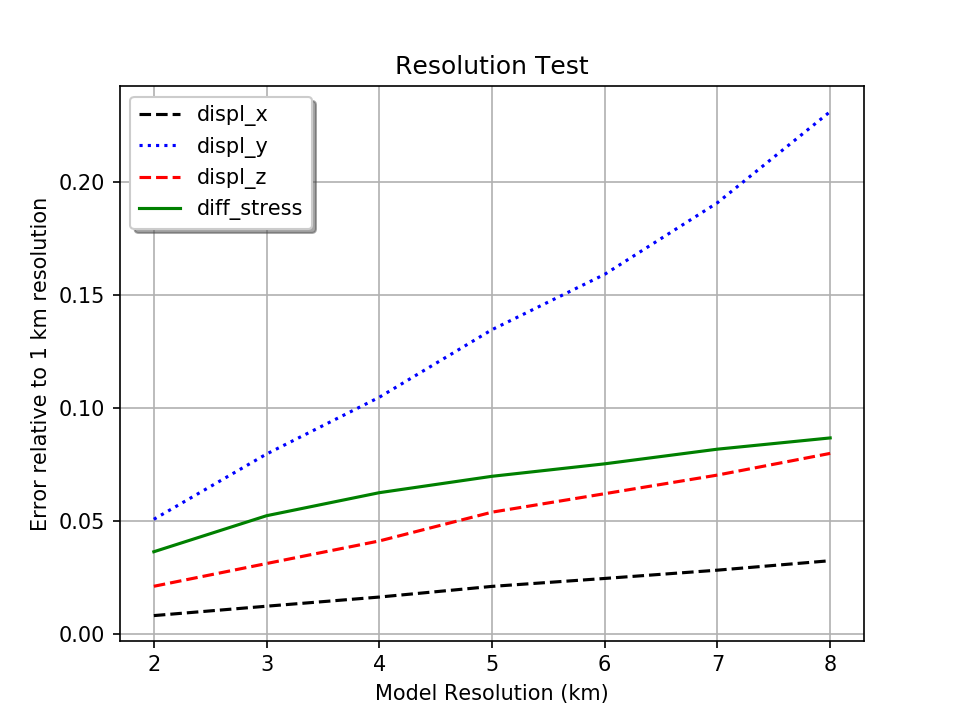
\includegraphics[width=25pc]{Figures/res_test_CSZ.png}
\caption{Errors in displacement components and differential stress ($\sigma_{D}$) for models with element sizes ranging from 2 to 8 km relative to a model with 1 km element size.}
\label{S1}
\end{sidewaysfigure}

\vspace{10mm} %5mm vertical space

This resolution test shows that the error generally increases with mesh resolution (Fig. \ref{S1}). %For example, the model has an error of about 0.02 and 0.16 in the $\sigma_{D}$ and $\phi_{\max}$ in element size of 2 km relative to 1 km, respectively (Fig. \ref{S2}). The error values increase to 0.06 and 0.26 when the element size is 4 km. 
The errors in displacement components and differential stress in models with element sizes of 2 km is less than 5 \% of the corresponding values in the model with 1 km resolution. The errors are less than 10 \% for models with element sizes below 4 km. In our study, we will use an element size of 2 km for our fault models. However, due to expensive computation time, we will use an element size of 4 km to evaluate model parameters, e.g., coefficient of friction.

\vspace{10mm} %5mm vertical space

\noindent\textbf{Stopping criterion of differential stress at 10 km depth}
\vspace{10mm} %5mm vertical space

\begin{sidewaysfigure}
\setfigurenum{S2}
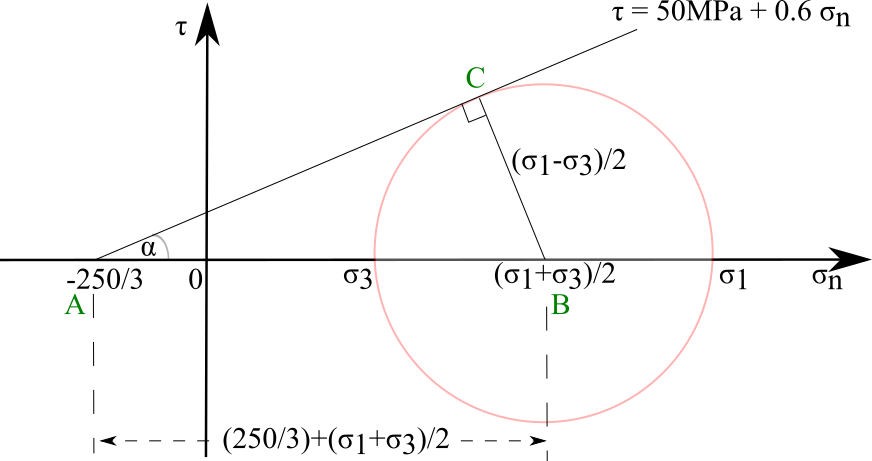
\includegraphics[width=25pc]{Figures/Calc_diff_stress.png}
\caption{Determining the differential stress for stopping criterion.}
\label{S2}
\end{sidewaysfigure}

\vspace{5mm} %5mm vertical space

From $\Delta$ABC,
\[
 \sin(\alpha) = \frac{\sigma_{1}-\sigma_{3}}{2}/[\frac{250}{3} + \frac{\sigma_{1}+\sigma_{3}}{2}],
\]
%
\[
 \sin(\alpha) = \frac{3(\sigma_{1}-\sigma_{3})}{3(\sigma_{1}+\sigma_{3})+500},
\]
%
\[
 \sigma_{1} = \frac{\sigma_{3}+[\sigma_{3}+\frac{500}{3}]\times \sin(\alpha)}{1-\sin(\alpha)},
\]

Based on Byerlee's law, $\tau$  = 50 MPa + 0.6$\,\sigma_n$, under the assumption of absence of pore-fluid pressure along the rift faults, $\tan(\alpha) = 0.6$, hence, $\sin(\alpha)= 0.5145$. $\sigma_{3}$ corresponds to the lithostatic stress, and assuming it is equal to 250 MPa at 10 km depth, gives $\sigma_{1}$ = 956.4882 MPa. Hence, the differential stress at 10 km depth with no pore-fluid pressure ($\sigma_{D} = \sigma_{1} - \sigma_{3})$ is 706.4882 MPa. 

\vspace{10mm} %5mm vertical space

\noindent\textbf{Effects of density ratio in the impact structure}

The percentage change in differential stress ($\Delta\sigma_{D}^{\prime}$), SH$_{\max}$ orientation ($\phi_{\max}$), and the change in $\phi_{\max}$ ($\Delta\phi_{\max}$) relative to the reference model (SNFR25) for models with different impact structure-crust density ratio.  The maps show no significant change with density ratio. We use density ratio of 10\% in this study to model a realistic damaged crustal rock. 
\vspace{10mm} %5mm vertical space

\begin{sidewaysfigure}
\setfigurenum{S3}
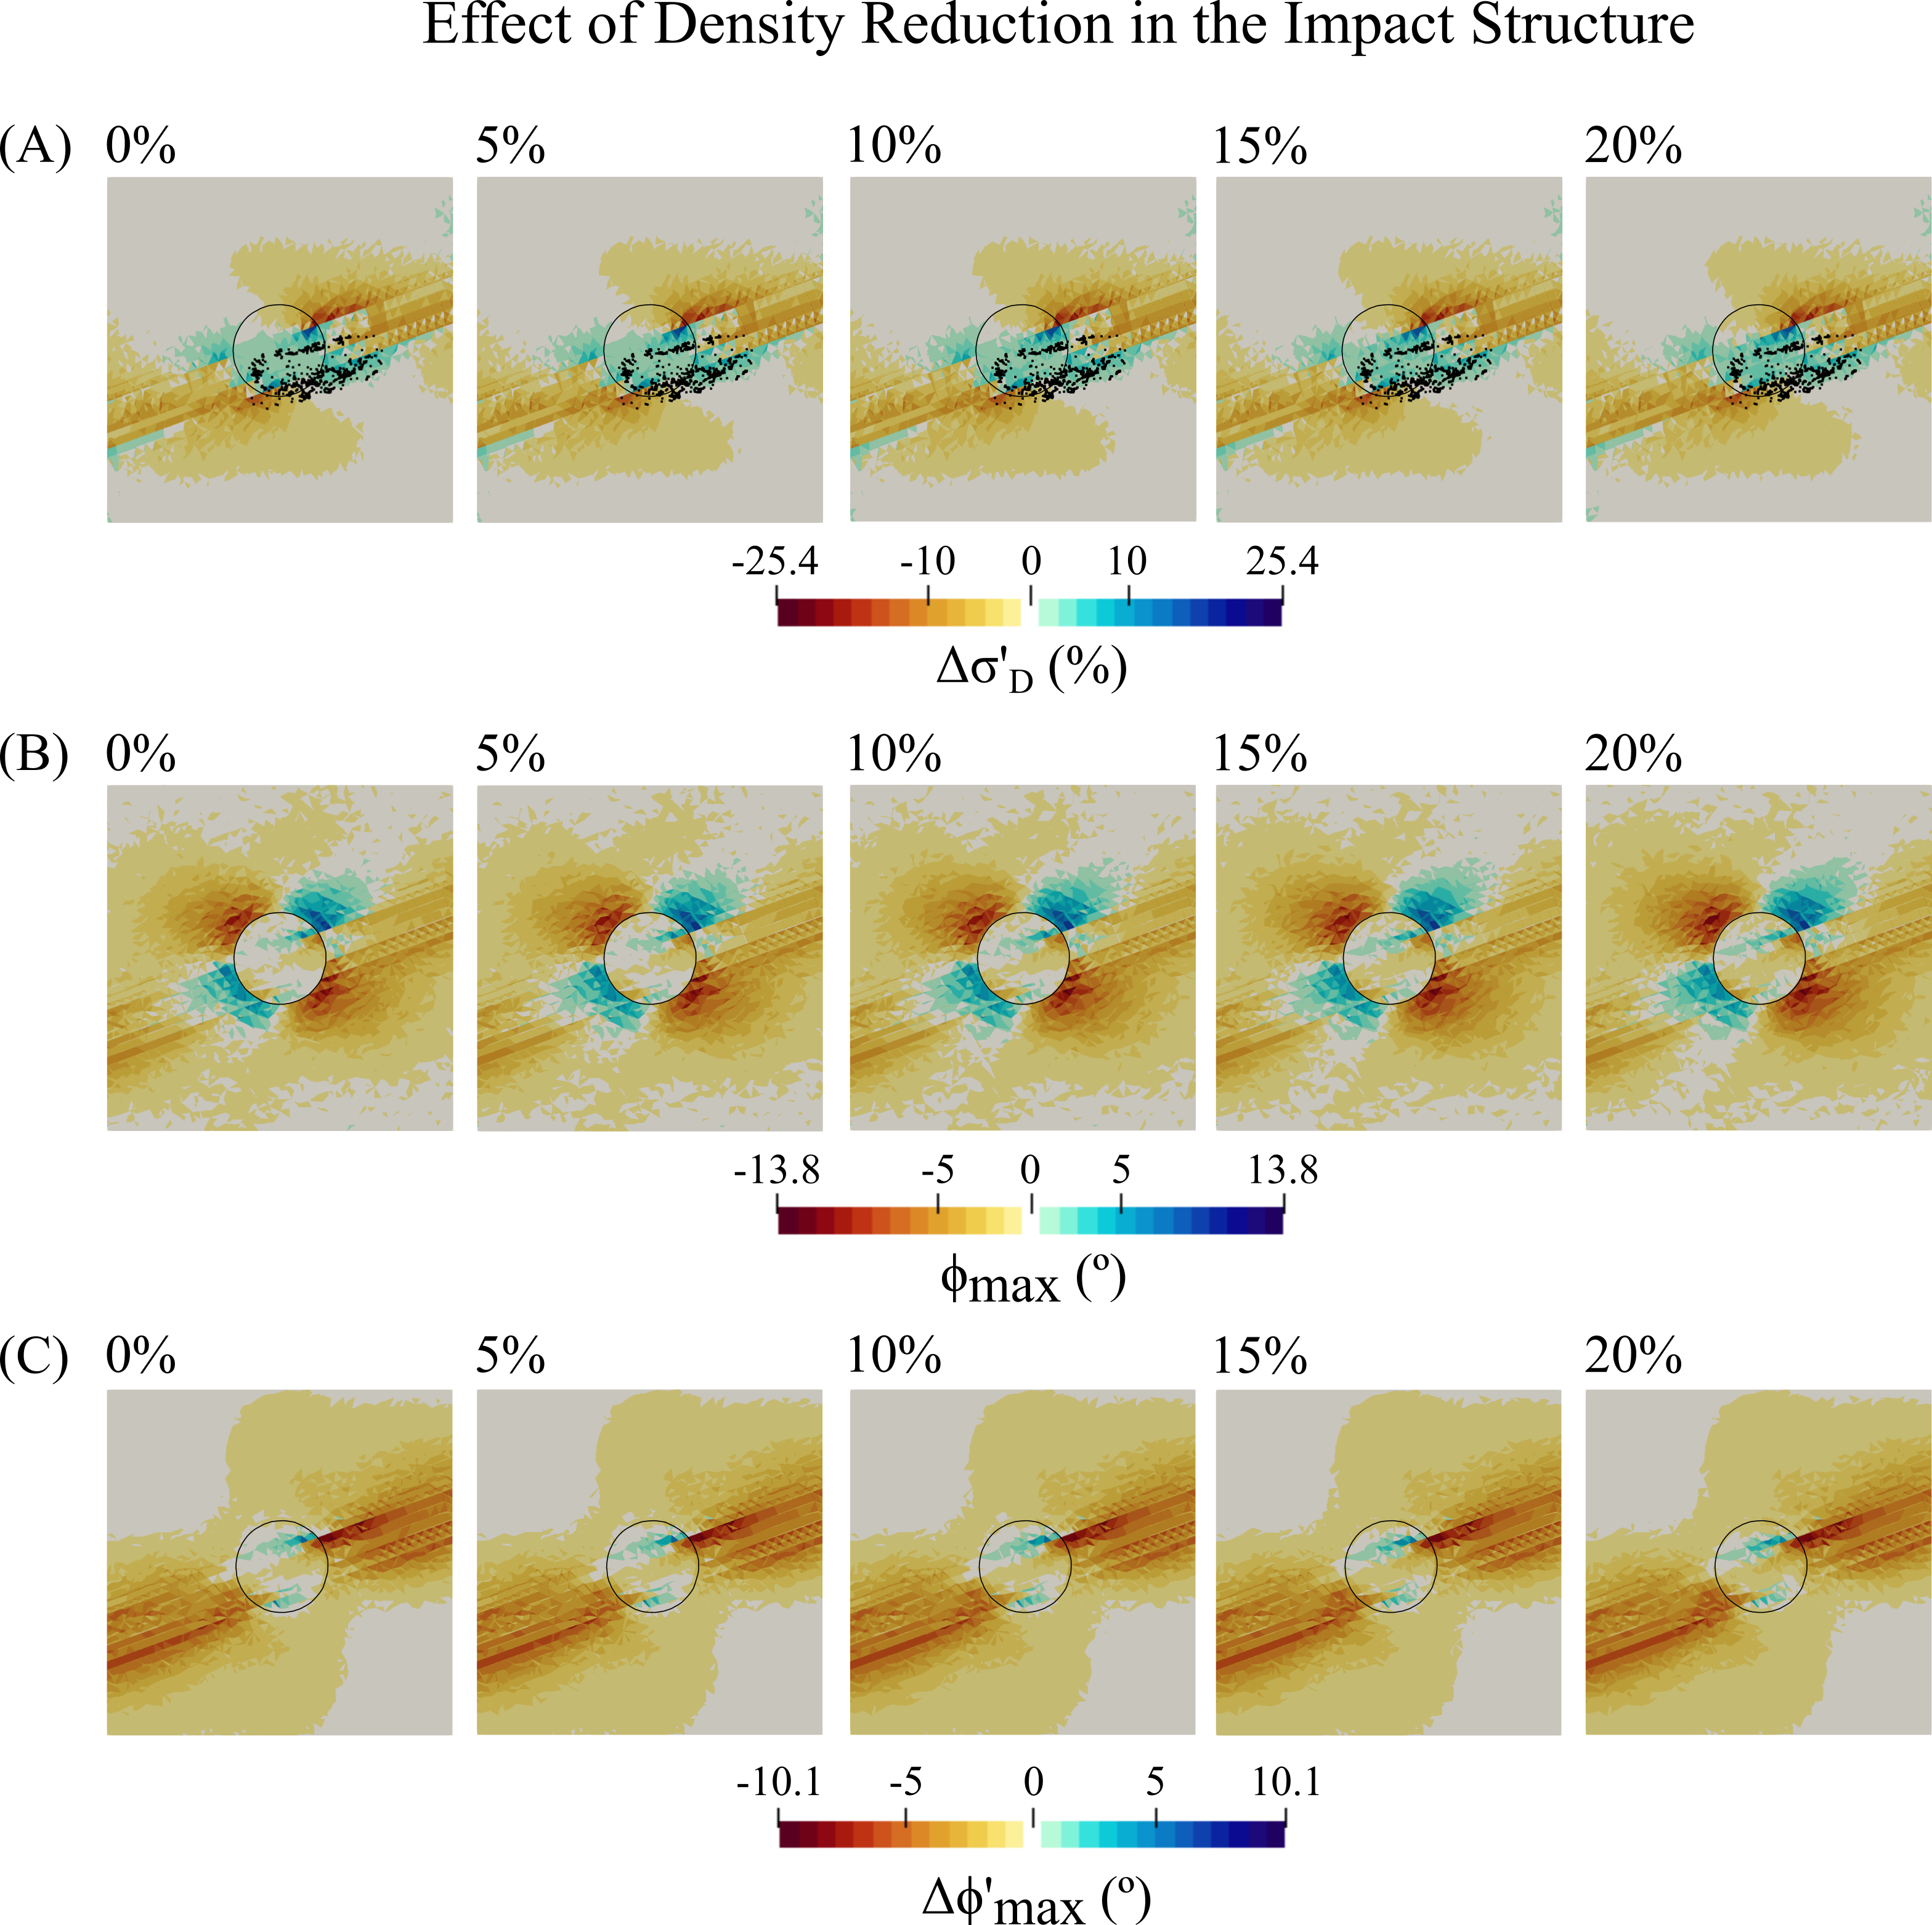
\includegraphics[width=25pc]{Figures/effect_of_density.png}
\caption{Effect of impact structure-crust density ratio on the $\Delta\sigma_{D}^{\prime}$, $\phi_{\max}$ and $\Delta \phi_{\max}^{\prime}$ at 10 km depth. Earthquakes within 2 km of each depth slice are represented by black dots in \ref{S3}A. The outline of the impact structure is represented as black circle. Each figure is 70 $\times$ 70 km.}
\label{S3}
\end{sidewaysfigure}

\vspace{10mm} %5mm vertical space

\noindent\textbf{Effect of cohesion}

We compute $\Delta \sigma_{D}^{\prime}$, $\phi_{\max}$ and $\Delta \phi_{\max}^{\prime}$ in a series of models in which the rift faults dip at 70$^{\circ}$ (i.e., SD70R25) but their cohesion ($C$) is varied systematically at a constant coefficient of friction ($\mu$) of 0.3. We assume that the fault parameters are the same for each rift fault and uniform throughout the fault surfaces. Six models with 0, 3, 5, 10, 20 and 30 MPa are constructed (Fig. \ref{S4}).

Magnitudes of $\Delta\sigma_D^{\prime}$ and $\phi_{\max}$ decrease with increasing cohesion. $\Delta\sigma_D^{\prime}$ maps spatially overlap with the distribution of seismicity at all the fault cohesions, especially well when the cohesion is less than 5 MPa (Fig. \ref{S4}A). However, the models could not explain some earthquakes in the SW corner of the crater. The $\Delta\sigma_D^{\prime}$ is not affected by a change in cohesion between 0 and 5 MPa. However, $\phi_{\max}$ approaches the reference no-fault model as the cohesion increases (Fig. \ref{S4}B). As cohesion increases, $\Delta\phi_{\max}$ decreases in value and the rotation is concentrated in the fault region outside the crater (Fig. \ref{S4}C). $\Delta\phi_{\max}$ is up to 10.8$^\circ$ when the cohesion is less than 5 MPa. 

Figure \ref{S4} shows that $\mu$ is an essential fault parameter needed to explain the seismicity of the CSZ because the value of $\mu$ affects the slope of the Mohr-Coulomb failure envelope. We use a cohesion value of 0 MPa to explain the spatial distribution of observed seismicity in the CSZ. 

\vspace{10mm} %5mm vertical space

\begin{sidewaysfigure}
\setfigurenum{S4}
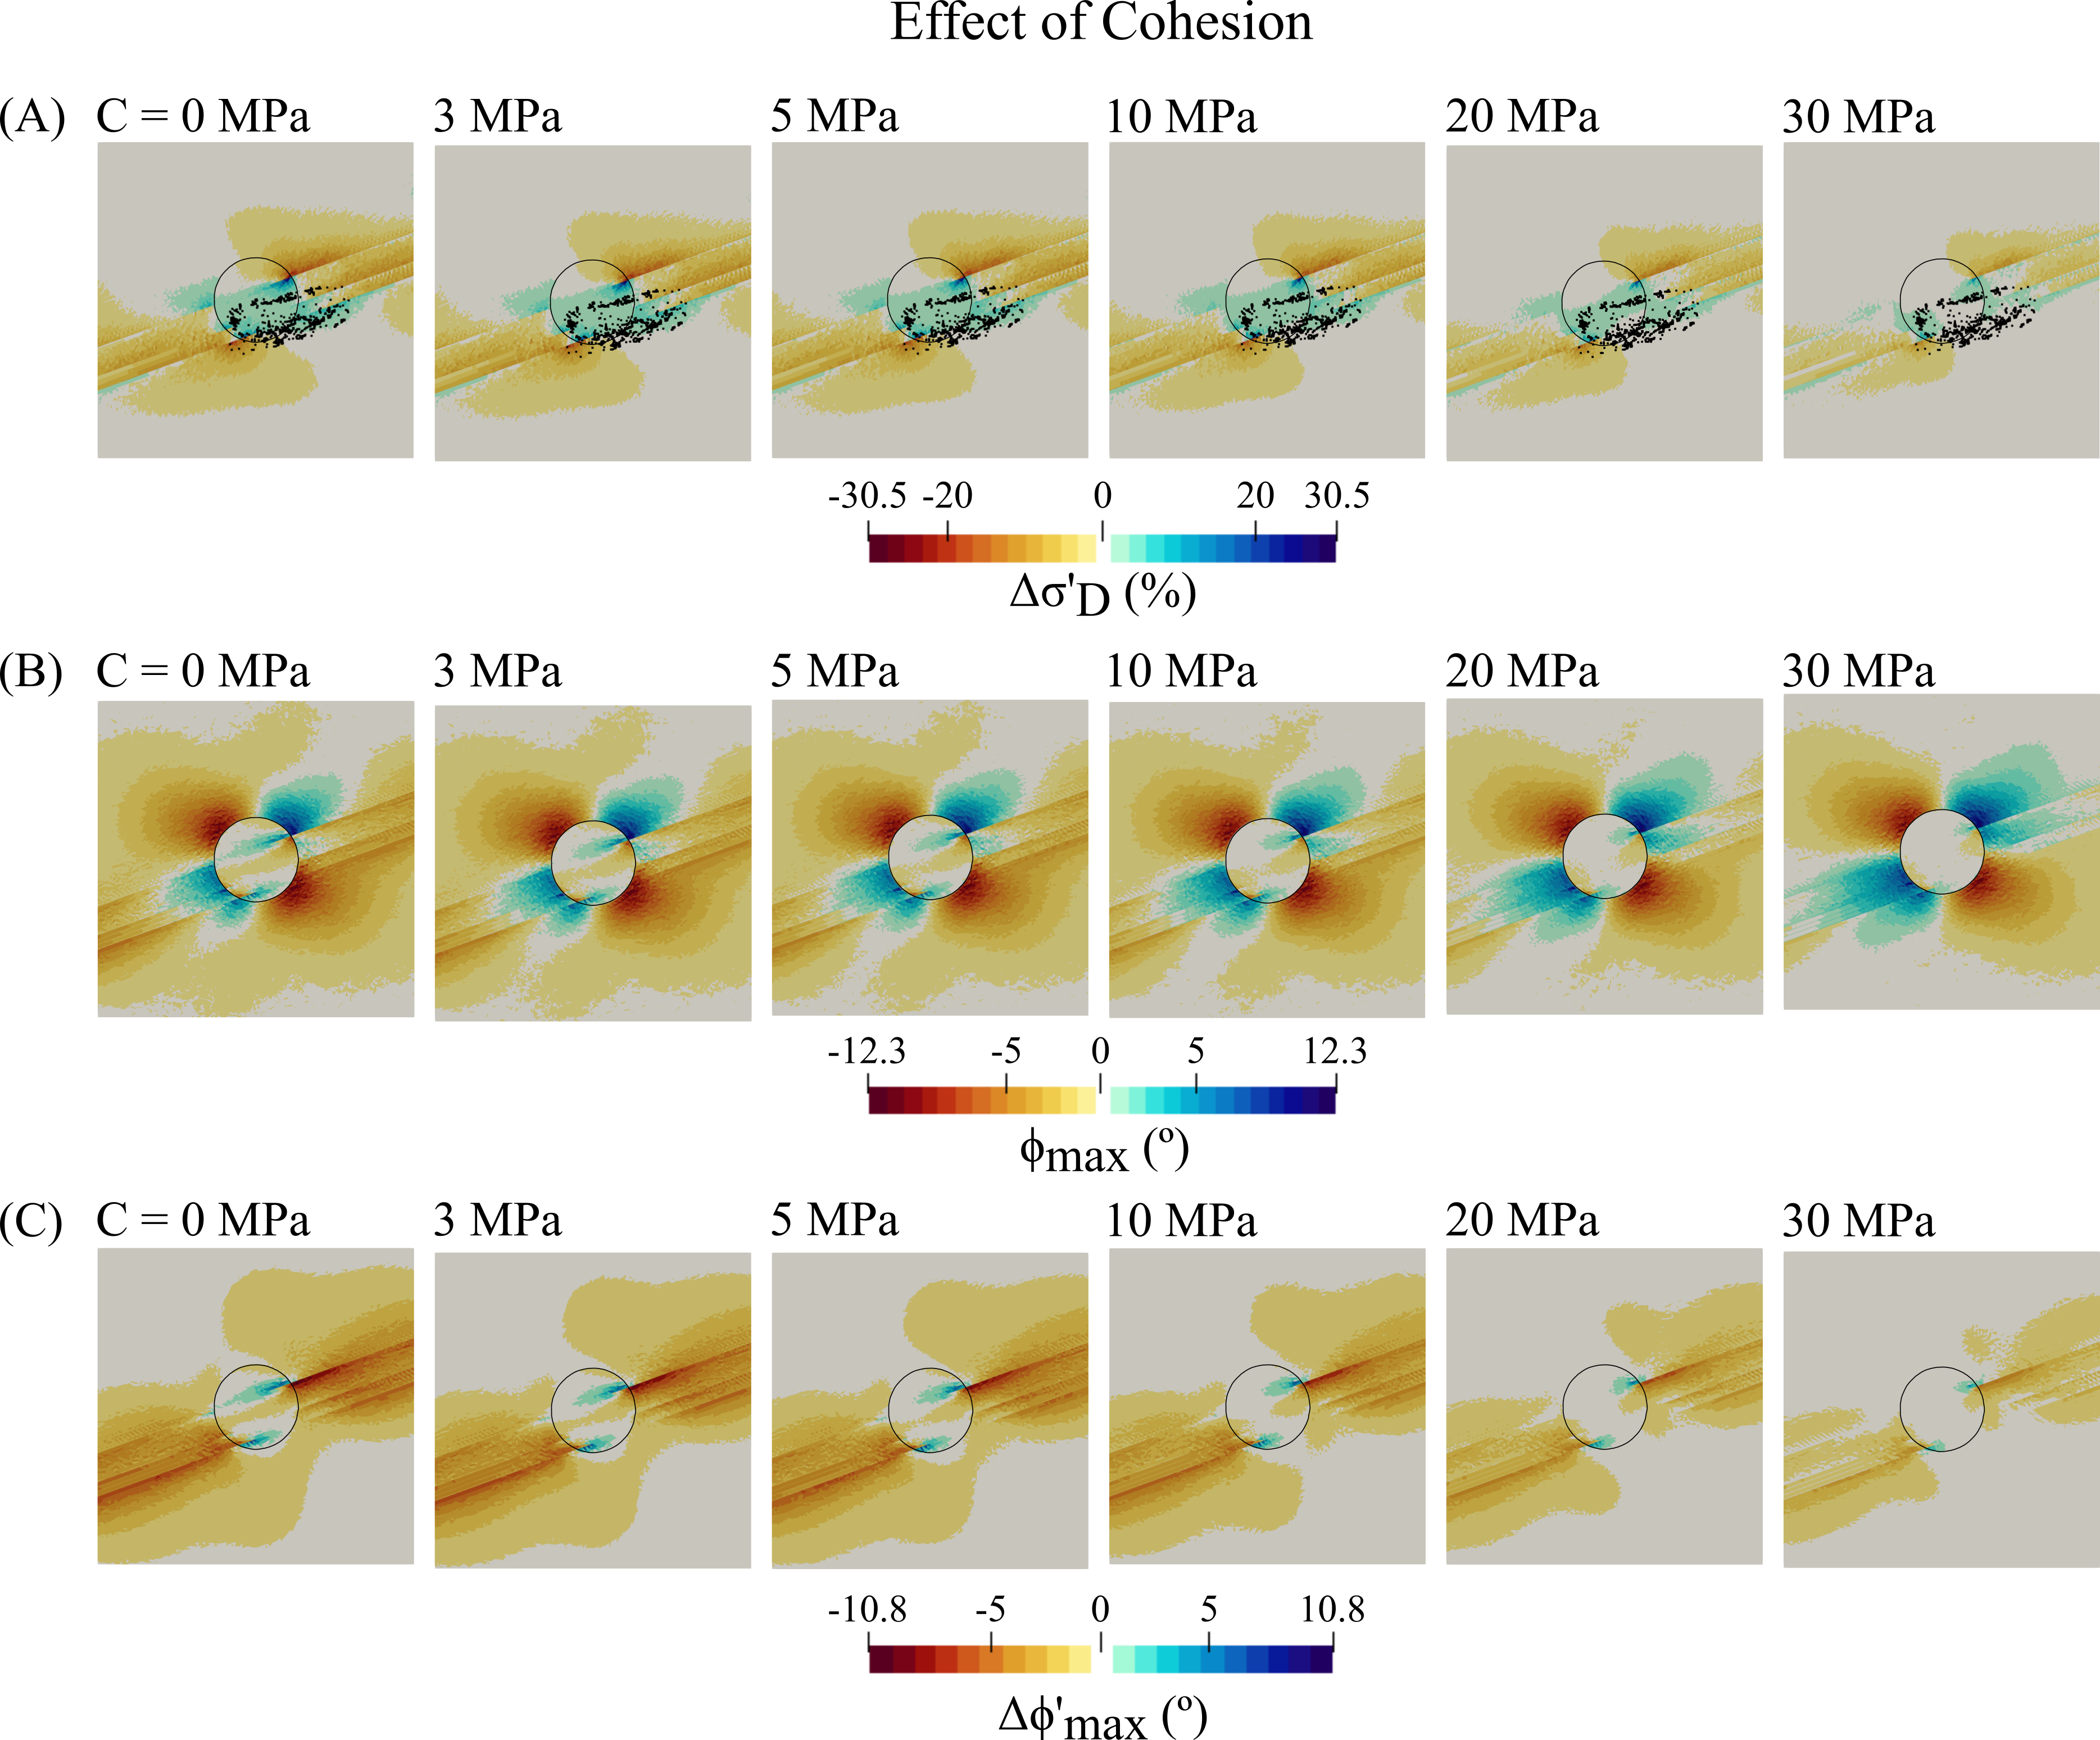
\includegraphics[width=25pc]{Figures/SD70R25C_S2.png}
\caption{Same as \ref{S3} but for the models with different cohesion values.}
\label{S4}
\end{sidewaysfigure}

\vspace{10mm} %5mm vertical space

\noindent\textbf{Effects of no impact structure (SD70R100 model)}

The percentage change in differential stress ($\Delta\sigma_{D}^{\prime}$), SH$_{\max}$ orientation ($\phi_{\max}$), and the change in $\phi_{\max}$ ($\Delta\phi_{\max}$) relative to the reference model (SNFR25) at various depths from the SD70R100 model.  $\Delta\sigma_{D}^{\prime}$ shows increased $\sigma_{D}$ relative to SNFR25 throughout the entire length of the rift faults at and below 15 km depth, hence the model predicts earthquakes in those regions. 

\vspace{10mm} %5mm vertical space

\begin{sidewaysfigure}
\setfigurenum{S5}
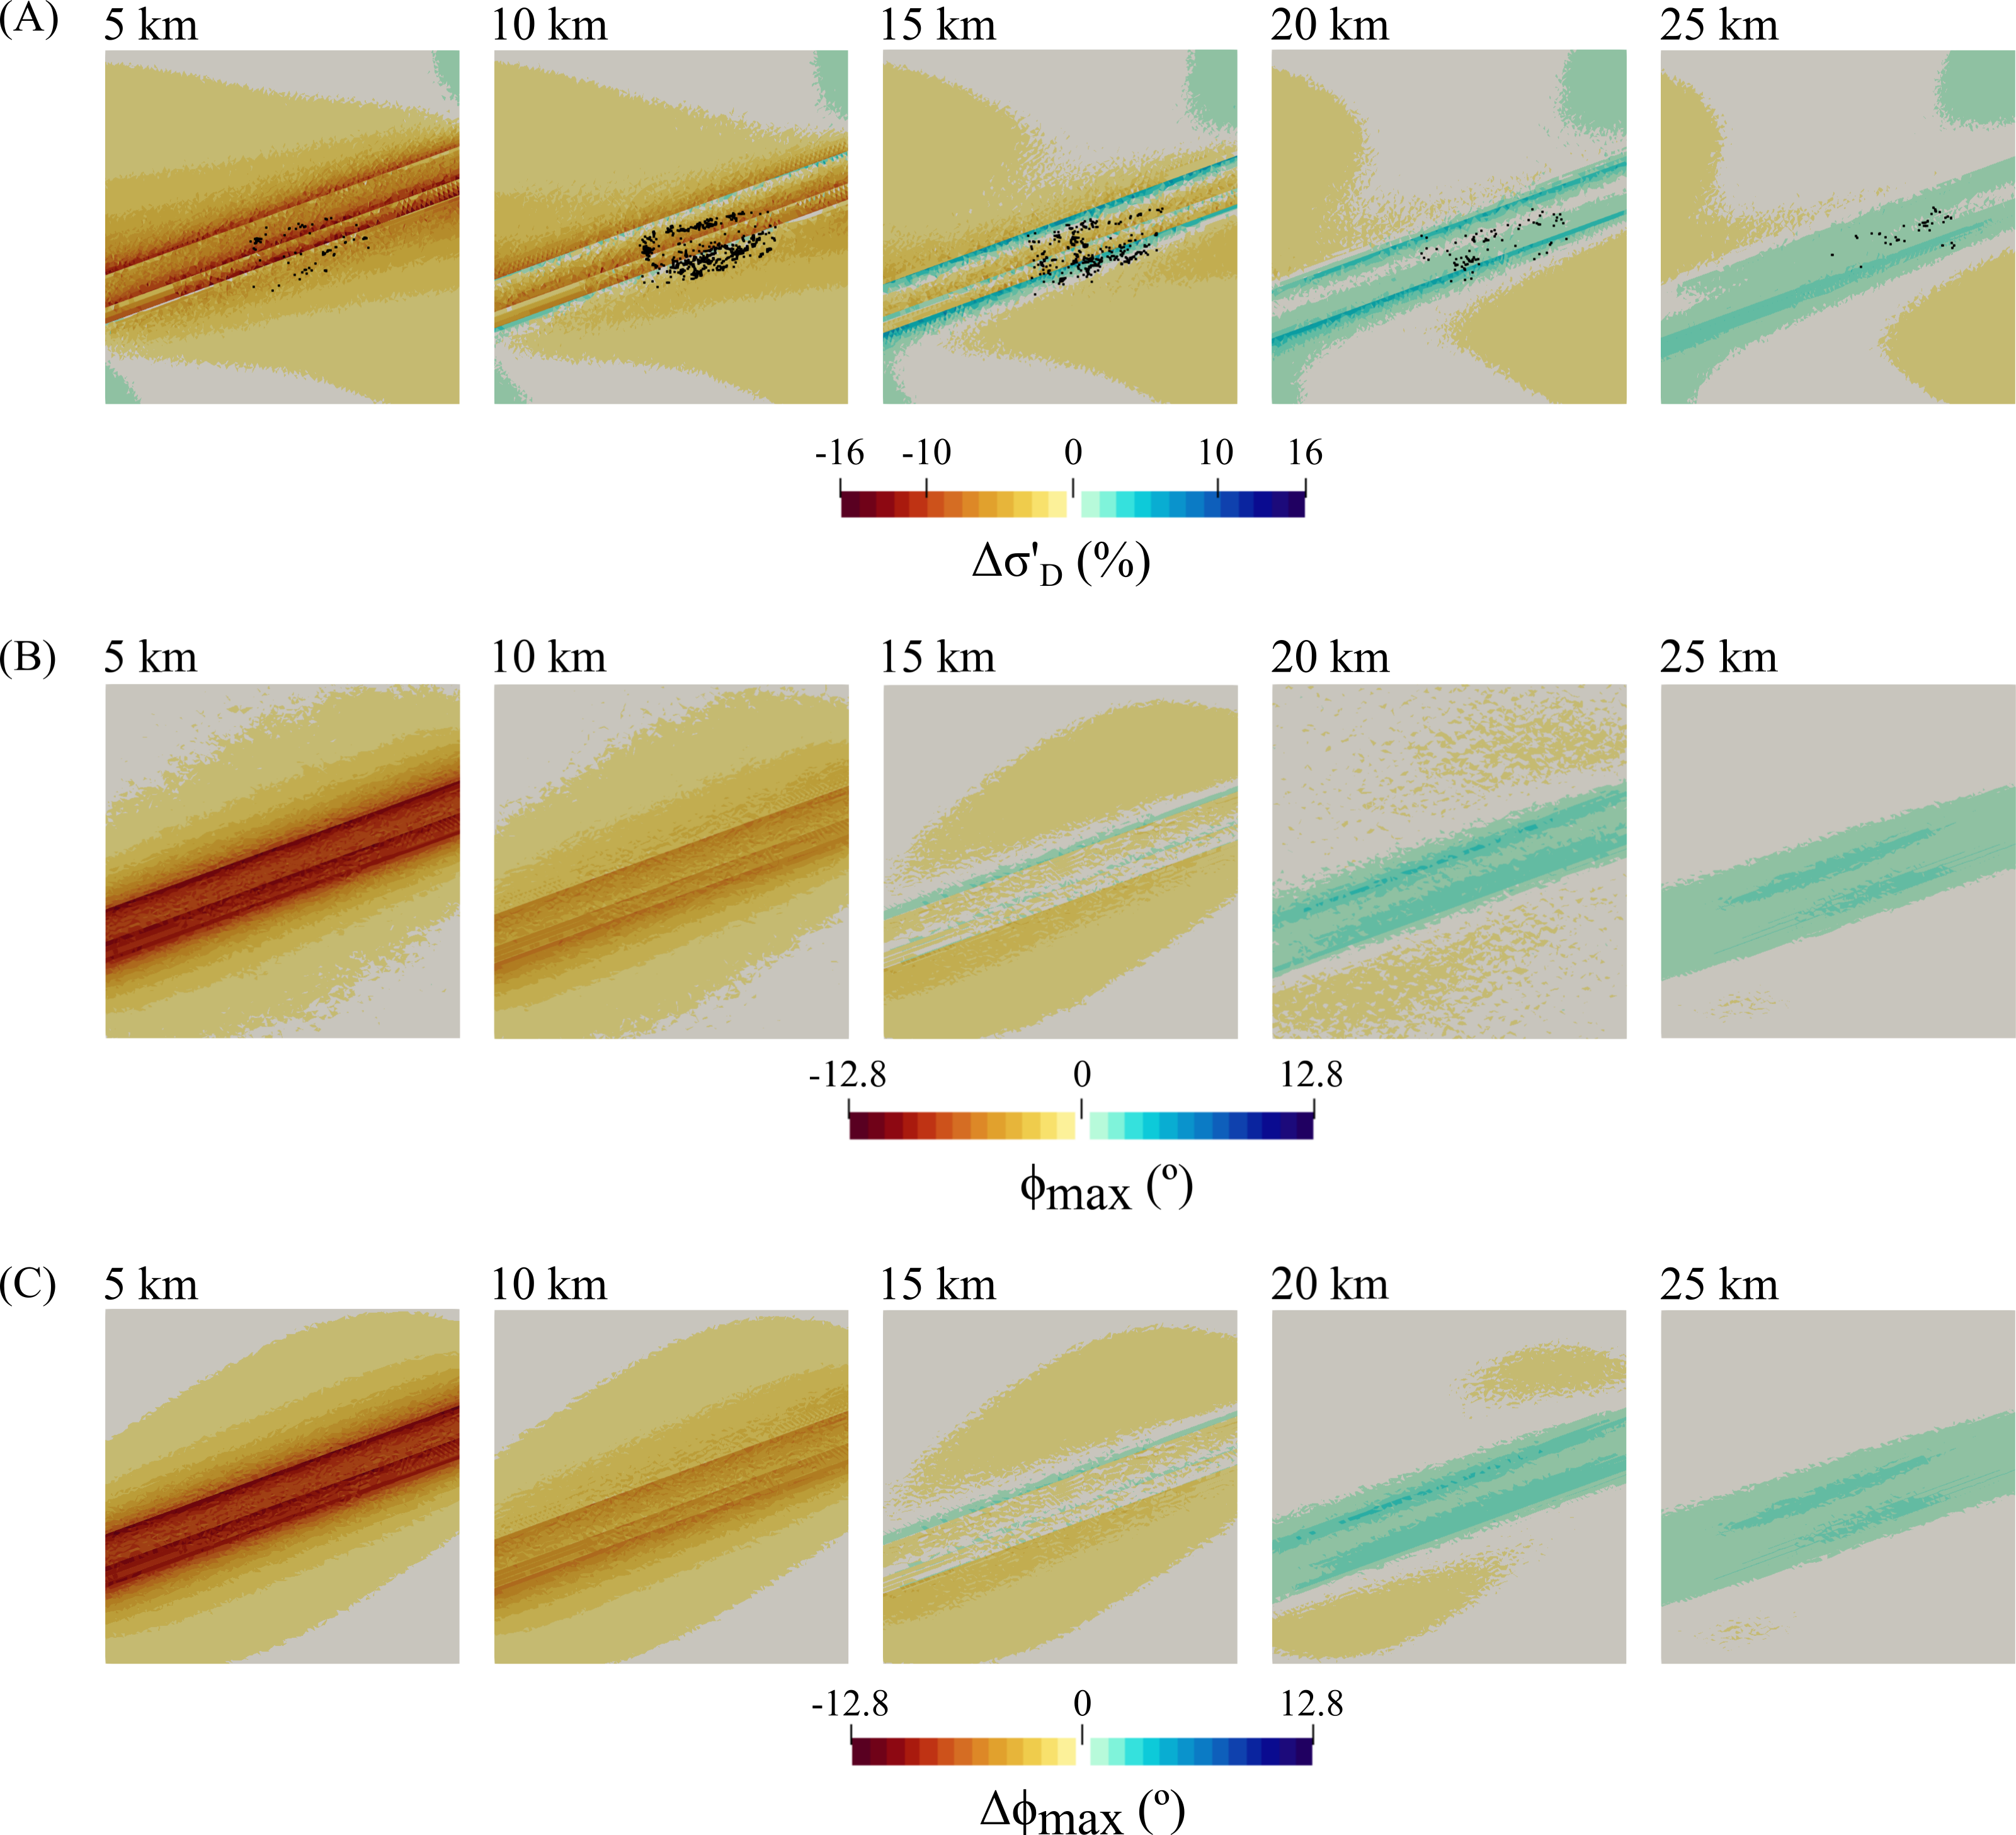
\includegraphics[width=25pc]{Figures/SD70R100_S1.png}
\caption{Percentage change in differential stress ($\Delta\sigma_{D}^{\prime}$), SH$_{\max}$ orientation ($\phi_{\max}$), and the change in $\phi_{\max}$ ($\Delta\phi_{\max}$) relative to the SNFR25 at various depths depths from the SD70R100 model. Earthquakes within 2 km of each depth slice are represented by black dots in \ref{S3}A. Each figure is 70 $\times$ 70 km.}
\label{S5}
\end{sidewaysfigure}

\vspace{10mm} %5mm vertical space
%\pagebreak


\noindent\textbf{Effects of impact structure-crust moduli ratio}

We test the response of the model results with different impact structure-crust moduli ratio. The model with a moduli ratio of 1.0 does not have the impact crater. The models show a better spatial correlation with the observed seismicity when the moduli ratio is 0.25. 

\vspace{10mm} %5mm vertical space

\begin{sidewaysfigure}
\setfigurenum{S6}
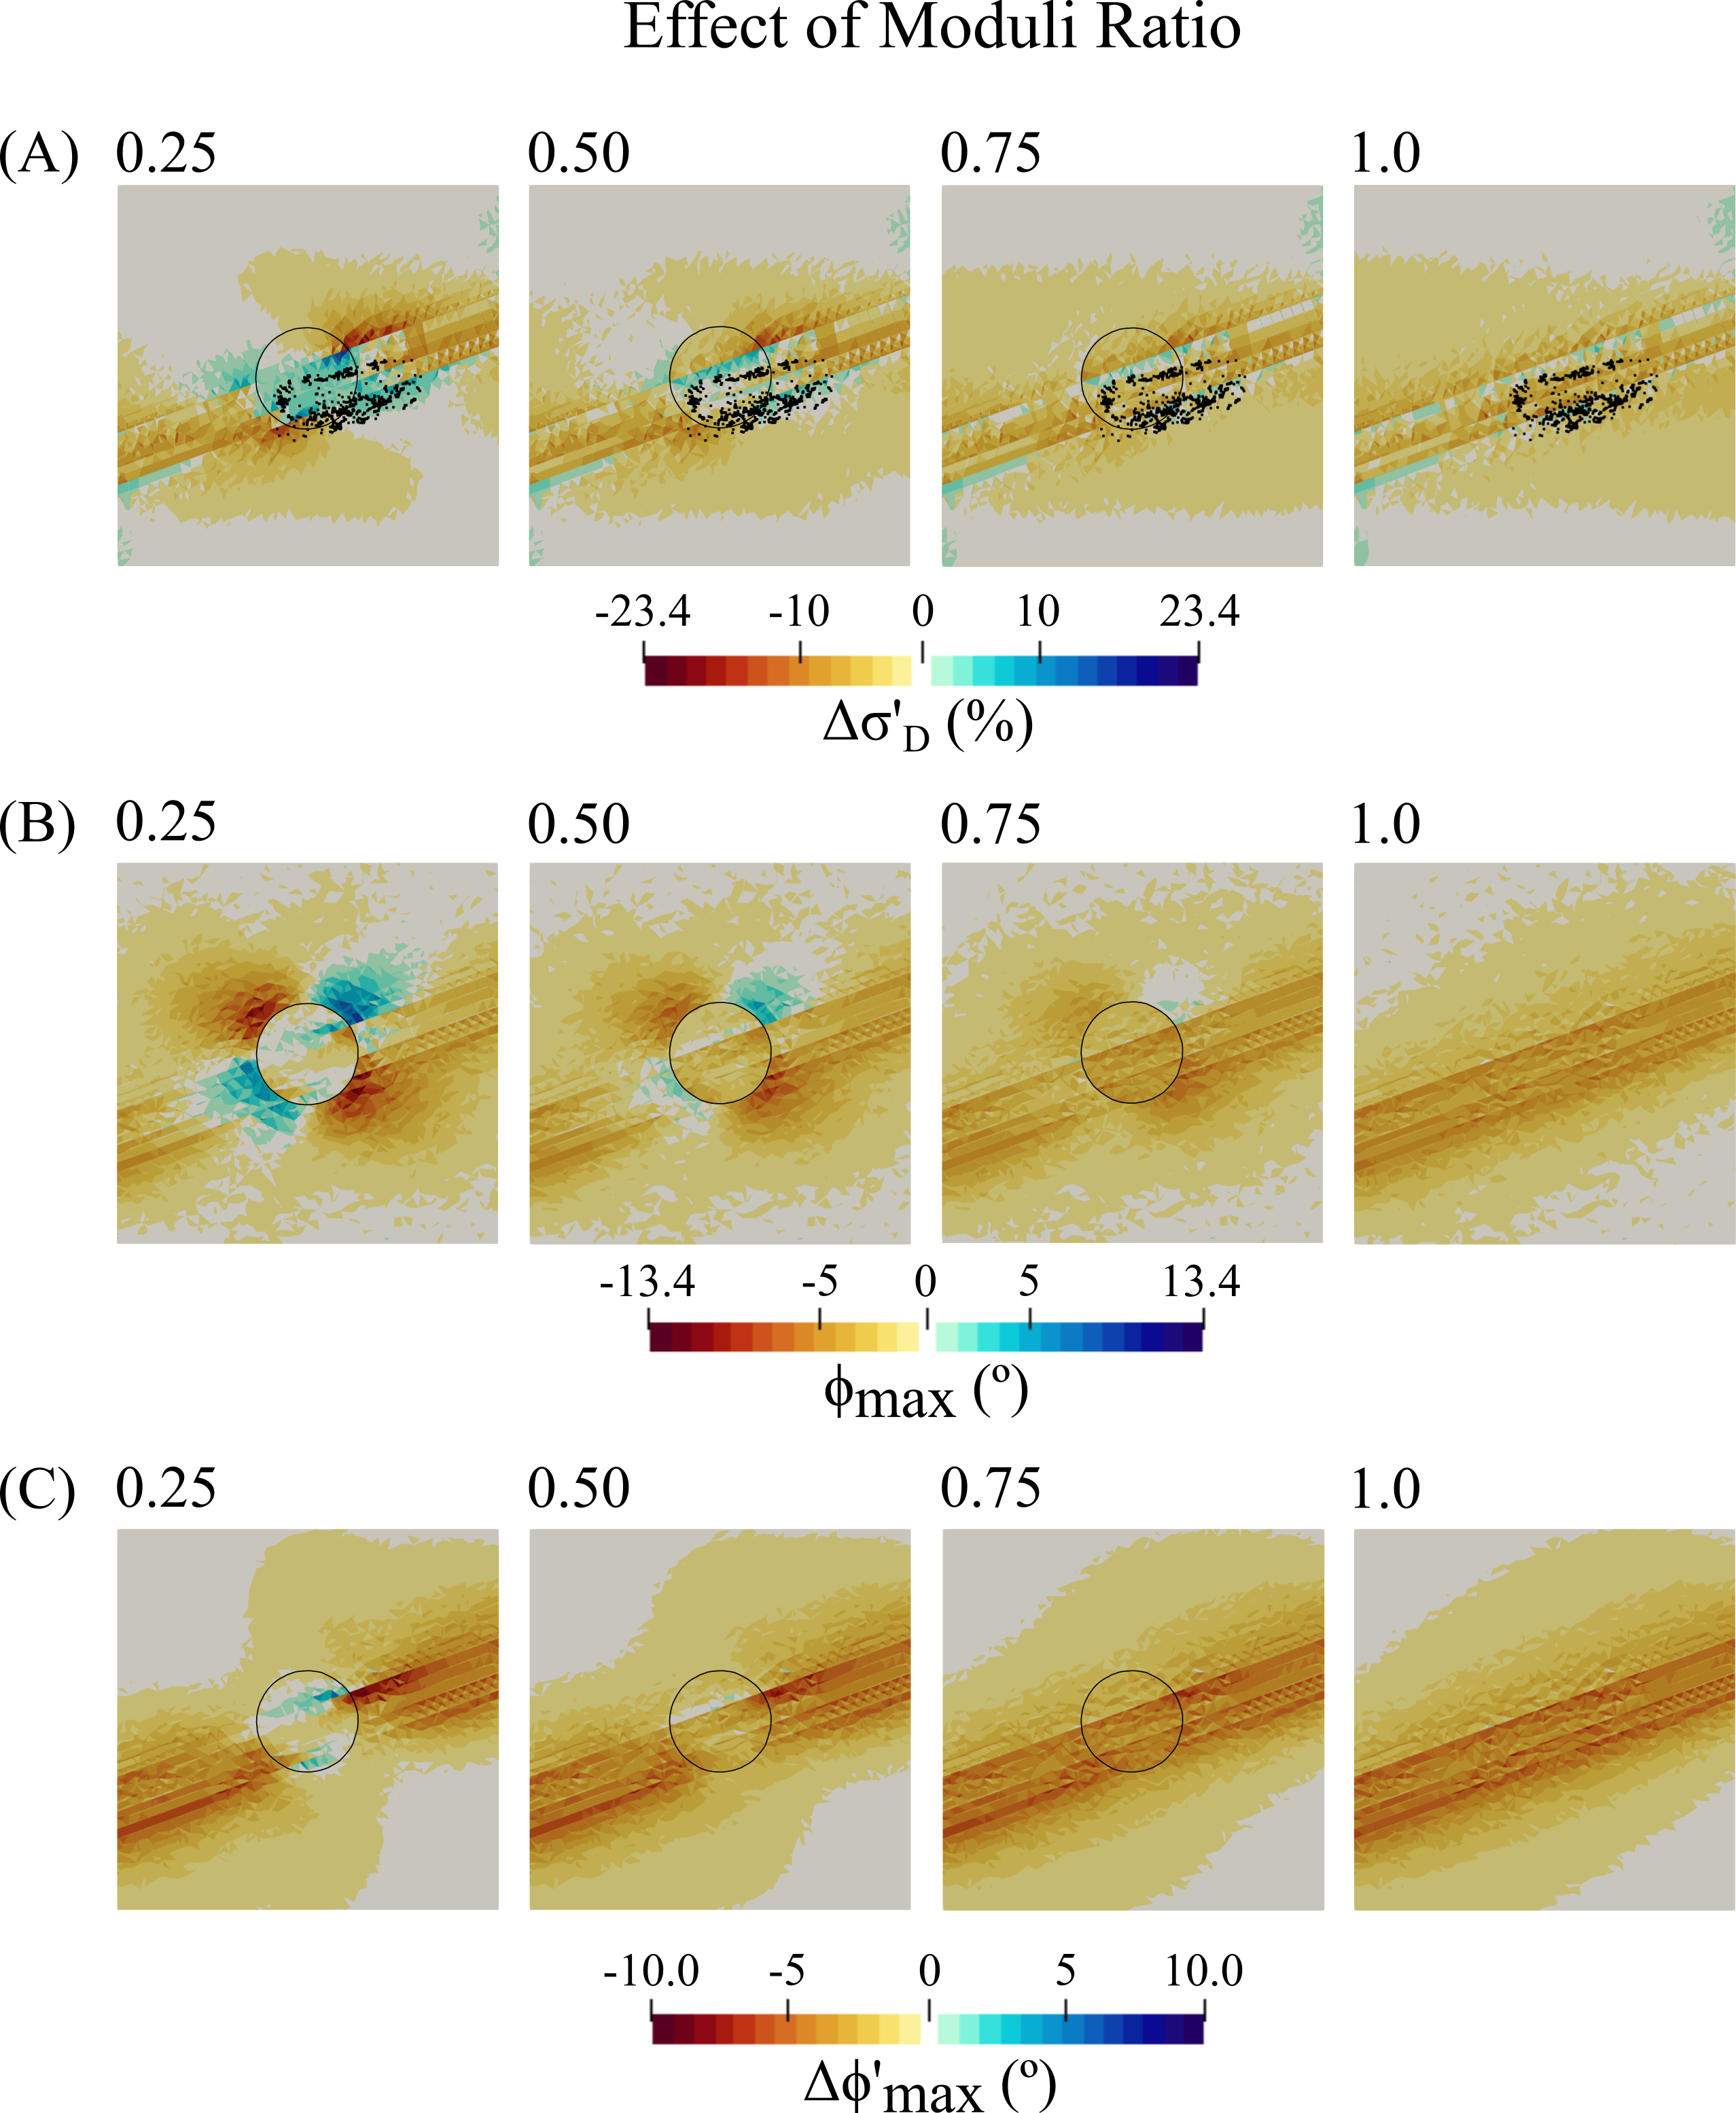
\includegraphics[width=25pc]{Figures/effect_of_moduli_ratio.png}
\caption{Same as \ref{S3} but for the models with different impact structure-crust moduli ratio.}
\label{S6}
\end{sidewaysfigure}

\vspace{10mm} %5mm vertical space

%\pagebreak


















%\begin{figure}
%\setfigurenum{S1} %%You can change number for each figure if you want, not required. "S" prepended automatically.
%\noindent\includegraphics[width=\textwidth]{Figures/SD70R100/F1_r10_m3_c0_sup.png}
%\caption{caption}
%\label{epsfiguresample}
%\end{figure}



%Delete all unused file types below. Copy/paste for multiples of each file type as needed.
%\noindent\textbf{Text S1.}

%Type or paste text here. This should be additional explanatory text, such as: extended descriptions of results, full details of models, extended lists of acknowledgements etc.  It should not be additional discussion, analysis, interpretation or critique. It should not be an additional scientific experiment or paper.
%
%Repeat for any additional Supporting Text

%%Enter Data Set, Movie, and Audio captions here
%%EXAMPLE CAPTIONS

%\noindent\textbf{Data Set S1.} %Type or paste caption here.
%upload your dataset(s) to AGU's journal submission site and select "Supporting Information (SI)" as the file type. Following naming %convention: ds01.

%Repeat for any additional Supporting data sets

%\noindent\textbf{Movie S1.} %Type or paste caption here.
%upload your movie(s) to AGU's journal submission site and select, "Supporting Information %(SI)" as the file type. Following naming convention: ms01.

%Repeat any additional Supporting movies

%\noindent\textbf{Audio S1.} %Type or paste caption here.
%upload your audio file(s) to AGU's journal submission site and select "Supporting Information %(SI)" as the file type. Following naming convention: auds01.


%Repeat for any additional Supporting audio files

%%% End of body of article:
%%%%%%%%%%%%%%%%%%%%%%%%%%%%%%%%%%%%%%%%%%%%%%%%%%%%%%%%%%%%%%%%
%
% Optional Notation section goes here
%
% Notation -- End each entry with a period.
% \begin{notation}
% Term & definition.\\
% Second term & second definition.\\
% \end{notation}
%%%%%%%%%%%%%%%%%%%%%%%%%%%%%%%%%%%%%%%%%%%%%%%%%%%%%%%%%%%%%%%%


%% ------------------------------------------------------------------------ %%
%%  REFERENCE LIST AND TEXT CITATIONS

%%%%%%%%%%%%%%%%%%%%%%%%%%%%%%%%%%%%%%%%%%%%%%%
% 
%
% \bibliography{<name of your .bib file>} do not specify file extension
%
% no need to specify bibliographystyle
%
% Note that ALL references in this supporting information file must also be referenced in the primary manuscript
%
%%%%%%%%%%%%%%%%%%%%%%%%%%%%%%%%%%%%%%%%%%%%%%%
% if you get an error about newblock being undefined, uncomment this line:
%\newcommand{\newblock}{}
%\bibliography{<name of your .bib file>} 




%Reference citation instructions and examples:
%
% Please use ONLY \cite and \citeA for reference citations.
% \cite for parenthetical references
% ...as shown in recent studies (Simpson et al., 2019)
% \citeA for in-text citations
% ...Simpson et al (2019) have shown...
% DO NOT use other cite commands (e.g., \citet, \citep, \citeyear, \nocite, \citealp, etc.).
%
%
%...as shown by \citeA{jskilby}.
%...as shown by \citeA{lewin76}, \citeA{carson86}, \citeA{bartoldy02}, and \citeA{rinaldi03}.
%...has been shown \cite{jskilbye}.
%...has been shown \cite{lewin76,carson86,bartoldy02,rinaldi03}.
%...has been shown \cite{lewin76,carson86,bartoldy02,rinaldi03}.
%
% DO NOT use other cite commands (e.g., \citet, \citep, \citeyear, \nocite, \citealp, etc.).
%

%% ------------------------------------------------------------------------ %%
%
%  END ARTICLE
%
%% ------------------------------------------------------------------------ %%
\end{article}
\clearpage

% Copy/paste for multiples of each file type as needed.

% enter figures and tables below here: %%%%%%%
%
%
%
%
% EXAMPLE FIGURES
% ---------------
% If you get an error about an unknown bounding box, try specifying the width and height of the figure with the natwidth and natheight options.
% \begin{figure}
%\setfigurenum{S1} %%You can change number for each figure if you want, not required. "S" prepended automatically.
% \noindent\includegraphics[natwidth=800px,natheight=600px]{samplefigure.eps}
%\caption{caption}
%\label{epsfiguresample}
%\end{figure}
%
%
% Giving latex a width will help it to scale the figure properly. A simple trick is to use \textwidth. Try this if large figures run off the side of the page.
% \begin{figure}
% \noindent\includegraphics[width=\textwidth]{anothersample.png}
%\caption{caption}
%\label{pngfiguresample}
%\end{figure}
%
%
%\begin{figure}
%\noindent\includegraphics[width=\textwidth]{athirdsample.pdf}
%\caption{A pdf test figure}
%\label{pdffiguresample}
%\end{figure}
%
% PDFLatex does not seem to be able to process EPS figures. You may want to try the epstopdf package.
%
%
% ---------------
% EXAMPLE TABLE
%
%\begin{table}
%\settablenum{S1} %%Change number for each table
%\caption{Time of the Transition Between Phase 1 and Phase 2\tablenotemark{a}}
%\centering
%\begin{tabular}{l c}
%\hline
% Run  & Time (min)  \\
%\hline
%  $l1$  & 260   \\
%  $l2$  & 300   \\
%  $l3$  & 340   \\
%  $h1$  & 270   \\
%  $h2$  & 250   \\
%  $h3$  & 380   \\
%  $r1$  & 370   \\
%  $r2$  & 390   \\
%\hline
%\end{tabular}
%\tablenotetext{a}{Footnote text here.}
%\end{table}
% ---------------
%
% EXAMPLE LARGE TABLE (UPLOADED SEPARATELY)
%\begin{table}
%\settablenum{S1} %%Change number for each table
%\caption{Time of the Transition Between Phase 1 and Phase 2\tablenotemark{a}}
%\end{table}


\end{document}

%%%%%%%%%%%%%%%%%%%%%%%%%%%%%%%%%%%%%%%%%%%%%%%%%%%%%%%%%%%%%%%

More Information and Advice:

%% ------------------------------------------------------------------------ %%
%
%  SECTION HEADS
%
%% ------------------------------------------------------------------------ %%

% Capitalize the first letter of each word (except for
% prepositions, conjunctions, and articles that are
% three or fewer letters).

% AGU follows standard outline style; therefore, there cannot be a section 1 without
% a section 2, or a section 2.3.1 without a section 2.3.2.
% Please make sure your section numbers are balanced.
% ---------------
% Level 1 head
%
% Use the \section{} command to identify level 1 heads;
% type the appropriate head wording between the curly
% brackets, as shown below.
%
%An example:
%\section{Level 1 Head: Introduction}
%
% ---------------
% Level 2 head
%
% Use the \subsection{} command to identify level 2 heads.
%An example:
%\subsection{Level 2 Head}
%
% ---------------
% Level 3 head
%
% Use the \subsubsection{} command to identify level 3 heads
%An example:
%\subsubsection{Level 3 Head}
%
%---------------
% Level 4 head
%
% Use the \subsubsubsection{} command to identify level 3 heads
% An example:
%\subsubsubsection{Level 4 Head} An example.
%
%% ------------------------------------------------------------------------ %%
%
%  IN-TEXT LISTS
%
%% ------------------------------------------------------------------------ %%
%
% Do not use bulleted lists; enumerated lists are okay.
% \begin{enumerate}
% \item
% \item
% \item
% \end{enumerate}
%
%% ------------------------------------------------------------------------ %%
%
%  EQUATIONS
%
%% ------------------------------------------------------------------------ %%

% Single-line equations are centered.
% Equation arrays will appear left-aligned.

Math coded inside display math mode \[ ...\]
 will not be numbered, e.g.,:
 \[ x^2=y^2 + z^2\]

 Math coded inside \begin{equation} and \end{equation} will
 be automatically numbered, e.g.,:
 \begin{equation}
 x^2=y^2 + z^2
 \end{equation}

% IF YOU HAVE MULTI-LINE EQUATIONS, PLEASE
% BREAK THE EQUATIONS INTO TWO OR MORE LINES
% OF SINGLE COLUMN WIDTH (20 pc, 8.3 cm)
% using double backslashes (\\).

% To create multiline equations, use the
% \begin{eqnarray} and \end{eqnarray} environment
% as demonstrated below.
\begin{eqnarray}
  x_{1} & = & (x - x_{0}) \cos \Theta \nonumber \\
        && + (y - y_{0}) \sin \Theta  \nonumber \\
  y_{1} & = & -(x - x_{0}) \sin \Theta \nonumber \\
        && + (y - y_{0}) \cos \Theta.
\end{eqnarray}

%If you don't want an equation number, use the star form:
%\begin{eqnarray*}...\end{eqnarray*}

% Break each line at a sign of operation
% (+, -, etc.) if possible, with the sign of operation
% on the new line.

% Indent second and subsequent lines to align with
% the first character following the equal sign on the
% first line.

% Use an \hspace{} command to insert horizontal space
% into your equation if necessary. Place an appropriate
% unit of measure between the curly braces, e.g.
% \hspace{1in}; you may have to experiment to achieve
% the correct amount of space.


%% ------------------------------------------------------------------------ %%
%
%  EQUATION NUMBERING: COUNTER
%
%% ------------------------------------------------------------------------ %%

% You may change equation numbering by resetting
% the equation counter or by explicitly numbering
% an equation.

% To explicitly number an equation, type \eqnum{}
% (with the desired number between the brackets)
% after the \begin{equation} or \begin{eqnarray}
% command.  The \eqnum{} command will affect only
% the equation it appears with; LaTeX will number
% any equations appearing later in the manuscript
% according to the equation counter.
%

% If you have a multiline equation that needs only
% one equation number, use a \nonumber command in
% front of the double backslashes (\\) as shown in
% the multiline equation above.

%% ------------------------------------------------------------------------ %%
%
%  SIDEWAYS FIGURE AND TABLE EXAMPLES
%
%% ------------------------------------------------------------------------ %%
%
% For tables and figures, add \usepackage{rotating} to the paper and add the rotating.sty file to the folder.
% AGU prefers the use of {sidewaystable} over {landscapetable} as it causes fewer problems.
%
% \begin{sidewaysfigure}
% \includegraphics[width=20pc]{samplefigure.eps}
% \caption{caption here}
% \label{label_here}
% \end{sidewaysfigure}
%
%
%
% \begin{sidewaystable}
% \caption{}
% \begin{tabular}
% Table layout here.
% \end{tabular}
% \end{sidewaystable}
%
%

